\documentclass{article}
\usepackage[utf8]{inputenc}
\usepackage{graphicx}
\usepackage{fancyhdr}
\usepackage{geometry}
\usepackage{amsmath}
\usepackage{amssymb}
\usepackage{url}
\usepackage{hyperref}
\usepackage{subcaption}

\geometry{left = 2cm, right=2cm, bottom=2cm, top=2cm}

\title{3806ICT - Maze Planning and Solving with Reinforcement Learning}
\author{Zac Jensen - s5153515 - zac.jensen@griffithuni.edu.au \\
    Jake Muggleton - s5130398 - jake.muggleton@griffithuni.edu.au}

\pagestyle{fancy}
\renewcommand{\headrulewidth}{1pt}
\fancyhf{}
\rhead{3806ICT - Maze Solving}
\chead{Griffith University}
\lhead{}
\rfoot{Page \thepage}
\newcommand\tab[1][1cm]{\hspace*{#1}}

\begin{document}
    \maketitle

%==============================================================================

    \section{Abstract}\label{sec:abstract}
        This reported aimed to analyze the differing ability between Q-learning 
        (a form of reinforcement learning) and CSP model checking using the 
        depth-first search (DFS) engine. Testing was conducted on mazes 
        ranging in size from 5x5 to 505x505, and the produced path length of 
        each method, along with the time taken for them to run, and their 
        memory usage, were evaluated. It was found that while CSP took a 
        significantly longer time to run and used more memory (exceeding the
        memory limit of the test system by 355x355), it always found a path
        to the goal, which Q-learning was unable to do. It was seen that 
        Q-learning tended to get 'stuck' while searching for the goal in a
        local optimum position, where it no longer has the ability to move 
        randomly enough to escape the local optimum, and so expends the rest 
        of its steps (up to maximum) in the same 1 or 2 states. It was concluded
        that, despite finding the same results while trying to manually 
        calibrate the Q-learning values, it is worth exploring different
        reward functions/algorithms to allow it to escape these local optima.

    \section{Introduction}\label{sec:introduction}
        Searching through a maze is a very complex task, because as the size 
        of the maze increases, the number of possible states increases 
        drastically. This makes it very difficult to find the 
        optimal solution in a reasonable amount of time.

        \tab Q-learning and CSP model checking using DFS are two very different 
        solutions to this maze search problem. Q-learning aims to search 
        for a path from start to goal using a reward function that guides 
        the algorithm, whereas CSP model checking using DFS is an exhaustive 
        search of possible paths to the goal.

        \tab One of the key differences between Q-learning and model checking is 
        that Q-learning is not guaranteed to find a path at all, whereas CSP 
        is able to find a path every single time. The downside of this is 
        that its runtime and memory usage can balloon quickly, and as maze 
        size increases it quickly becomes impractical to use.

    \section{Test Design}\label{sec:test-design}
        For this report, the designed test was to randomly generate mazes of 
        size 5x5 to size 505x505 and profile the running of both PAT analyzing 
        it with CSP in DFS mode and Q-learning. This allowed comparison of 
        the time taken for it to run, the length of the path it found, and 
        the memory it used to do so.

        \tab As for the implementation of these, the maze generator utilised a
        backtracking algorithm in $C++$, the CSP had an adjustment that marked its
        previous moves, and the reinforcement learning was the lab's version
        split into scripts. The reason for the maze using backtracking and being
        so optimised is because we want to be able to speed up generating
        samples. Furthermore, backtracking gives us a good time, memory,
        produced minimal dead ends, is bias free and not uniform 
        \cite{source}.

        \tab In terms of the hardware and software configuration, it was ran on
        WSL2 inside of Windows 10 on a Ryzen 5900 with 32GB of RAM. Due to it
        being in WSL2, mono was used to run PAT 3 which means that the times are
        likely around three times slower than they would be on just Windows. 
        The reason for using WSL2 is because we have access to the time command,
        which makes recording the memory of the reinforcement learning script
        easier. 

        \tab With regards to the parameters of the RL, it was set to be at 
        gamma$=0.99$, alpha=$0.1$, epsilon=$0.1$, max iterations to be 100 
        and maximum steps were 1000. This means that no solutions were found
        over 1000, but that's fine for this purpose.

    \section{Results}\label{sec:results}

        \begin{table}[ht!]
            \resizebox{\textwidth}{!}{
                % Since the table is so huge, its going to be easier for me to just make a whole
% separate file that contains the table
\begin{tabular}{|l||l|l|l||l|l|l|}
\hline
Size & CSP Path Length & CSP Time Taken (sec) & CSP Memory Usage (KB) & RL Path Length & RL
Time Taken (sec) & RL Memory Usage (KB) \\ 
\hline \hline
5    & 3               & 0.0125483      & 8691.928         & 5              & 0.42          & 52476           \\ \hline
15   & 5               & 0.0149705      & 12324.304        & 23             & 1.56          & 52692           \\ \hline
25   & 31              & 0.0264754      & 13624.272        & 41             & 2.41          & 52732           \\ \hline
35   & 189             & 0.0504123      & 13854.6          & 33             & 2.36          & 52772           \\ \hline
45   & 385             & 0.1140375      & 23686.088        & 103            & 6.18          & 52924           \\ \hline
55   & 883             & 0.2224756      & 47826.784        & N/A            & 21.05         & 53228           \\ \hline
65   & 779             & 0.3070878      & 66045.064        & 5              & 0.4           & 52364           \\ \hline
75   & 725             & 0.4824123      & 64616.464        & 85             & 8.41          & 53272           \\ \hline
85   & 429             & 1.2390332      & 206209.072       & N/A            & 22.65         & 53208           \\ \hline
95   & 775             & 0.6181151      & 95940.288        & 385            & 20.8          & 53048           \\ \hline
105  & 237             & 0.1414343      & 44906.904        & N/A            & 20.51         & 53268           \\ \hline
115  & 1153            & 2.8849482      & 571280.384       & N/A            & 20.82         & 52880           \\ \hline
125  & 2207            & 1.9307304      & 446417.984       & N/A            & 20.41         & 53692           \\ \hline
135  & 1935            & 5.3970906      & 467968.992       & N/A            & 20.73         & 53652           \\ \hline
145  & 2845            & 3.9961035      & 777228.416       & N/A            & 21.06         & 53560           \\ \hline
155  & 3067            & 13.6618017     & 2025940.864      & N/A            & 21.08         & 53708           \\ \hline
165  & 493             & 0.8841495      & 269999.168       & N/A            & 20.11         & 54148           \\ \hline
175  & 2245            & 13.6013149     & 1097147.648      & N/A            & 21.01         & 54100           \\ \hline
185  & 5325            & 26.767407      & 2554897.152      & N/A            & 20.92         & 54132           \\ \hline
195  & 7691            & 25.5085239     & 5052180.992      & N/A            & 20.85         & 54504           \\ \hline
205  & 7235            & 34.9948211     & 4563559.424      & N/A            & 21.65         & 54196           \\ \hline
215  & 2549            & 11.3362358     & 4005557.76       & N/A            & 20.96         & 54712           \\ \hline
225  & 1023            & 49.2342707     & 12712168.448     & N/A            & 20.43         & 54900           \\ \hline
235  & 8167            & 40.2563064     & 6696100.352      & N/A            & 21.05         & 54856           \\ \hline
245  & 6075            & 75.8756731     & 12245105.664     & N/A            & 20.22         & 55404           \\ \hline
255  & 8097            & 41.0211563     & 14666722.304     & N/A            & 21.23         & 55688           \\ \hline
265  & 9415            & 58.0503016     & 15315657.728     & N/A            & 20.69         & 55872           \\ \hline
275  & 10217           & 59.8128569     & 15368540.16      & N/A            & 20.28         & 56248           \\ \hline
285  & 3293            & 19.6668813     & 4052617.728      & N/A            & 20.68         & 56504           \\ \hline
295  & 11063           & 143.4064528    & 17374568.448     & 357            & 18.88         & 56752           \\ \hline
305  & 12619           & 112.3534874    & 17285484.544     & N/A            & 20.33         & 57380           \\ \hline
315  & 2415            & 17.9483529     & 4523416.576      & N/A            & 21.37         & 57380           \\ \hline
325  & 13693           & 137.4000611    & 24939696.128     & N/A            & 20.2          & 57716           \\ \hline
335  & 2847            & 18.7191763     & 4038628.352      & N/A            & 20.64         & 57848           \\ \hline
345  & 6807            & 607.3551285    & 28047468.544     & N/A            & 20.79         & 58004           \\ \hline
355  & 10275           & 119.7228921    & 21051107.328     & N/A            & 20.69         & 58088           \\ \hline
365  & N/A             & N/A            & N/A              & N/A            & 21.01         & 58772           \\ \hline
375  & N/A             & N/A            & N/A              & N/A            & 20.14         & 58944           \\ \hline
385  & N/A             & N/A            & N/A              & N/A            & 20.83         & 59756           \\ \hline
395  & N/A             & N/A            & N/A              & N/A            & 20.52         & 59384           \\ \hline
405  & N/A             & N/A            & N/A              & N/A            & 20.9          & 59716           \\ \hline
415  & N/A             & N/A            & N/A              & N/A            & 20.49         & 60272           \\ \hline
425  & N/A             & N/A            & N/A              & N/A            & 21.09         & 60512           \\ \hline
435  & N/A             & N/A            & N/A              & N/A            & 20.39         & 60264           \\ \hline
445  & N/A             & N/A            & N/A              & N/A            & 20.65         & 60724           \\ \hline
455  & N/A             & N/A            & N/A              & N/A            & 21.46         & 61720           \\ \hline
465  & N/A             & N/A            & N/A              & N/A            & 20.5          & 61328           \\ \hline
475  & N/A             & N/A            & N/A              & N/A            & 21.0          & 63628           \\ \hline
485  & N/A             & N/A            & N/A              & N/A            & 21.07         & 63248           \\ \hline
495  & N/A             & N/A            & N/A              & N/A            & 20.87         & 62624           \\ \hline
505  & N/A             & N/A            & N/A              & N/A            & 20.81         & 62940           \\ \hline
\end{tabular}
            }
        \end{table}
        \newpage


        \begin{figure}[ht]
            \begin{subfigure}{.5\textwidth}
                \centering
                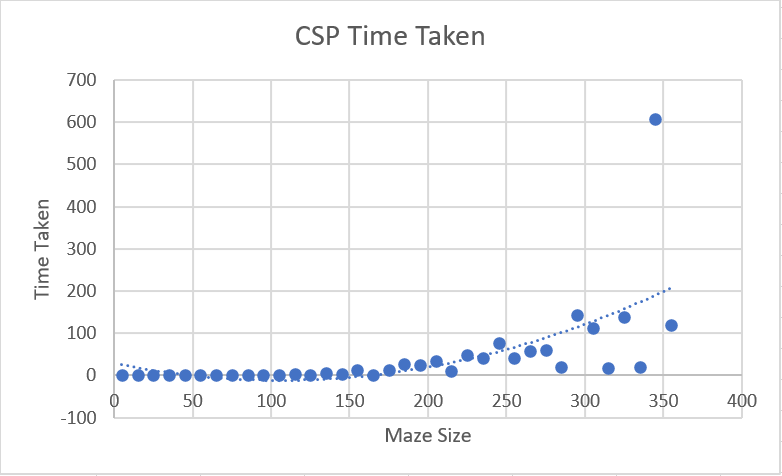
\includegraphics[scale=0.5]{assets/CSPTimeVsSize.PNG}
                \caption{Model checking time vs size}
            \end{subfigure}
            \begin{subfigure}{.5\textwidth}
                \centering
                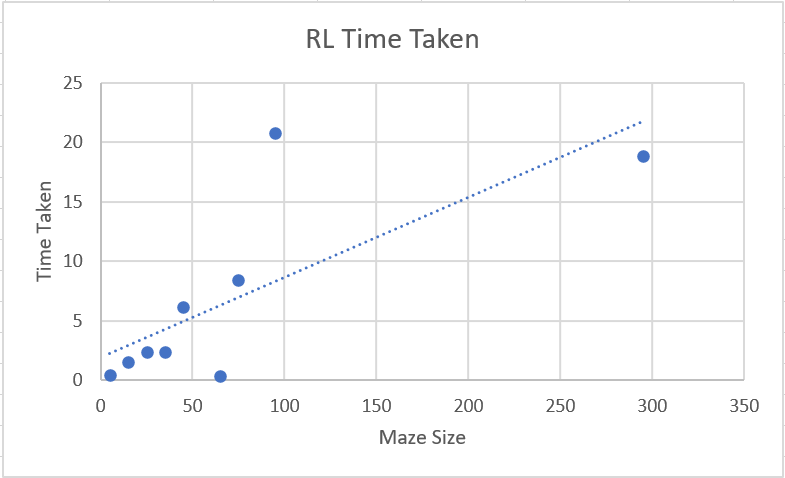
\includegraphics[scale=0.5]{assets/RLTimeVsSize.PNG}
                \caption{RL time vs size}
            \end{subfigure}
        \end{figure}

         \tab It can be seen from this figure that, when it successfully found a 
         path, reinforcement learning was much quicker than CSP, following a 
         time trend closer to $O(n)$. This is likely because the number of
         iterations is a constant, and actually if we look at the table we can
         see that the time spent trying to solve something is constant. 

         \tab CSP, on the other hand, followed a polynomial curve, somewhat 
         following a trend of $O(n^2)$. This makes sense because CSP 
         uses DFS, which would be $O(|V|+|E|)$ where $V$ is vertices (number 
         of cells in the graph, which is $n^2$) and $E$ is edges (which is 
         more or less constant).

        \begin{figure}[ht]
            \begin{subfigure}{.5\textwidth}
                \centering
                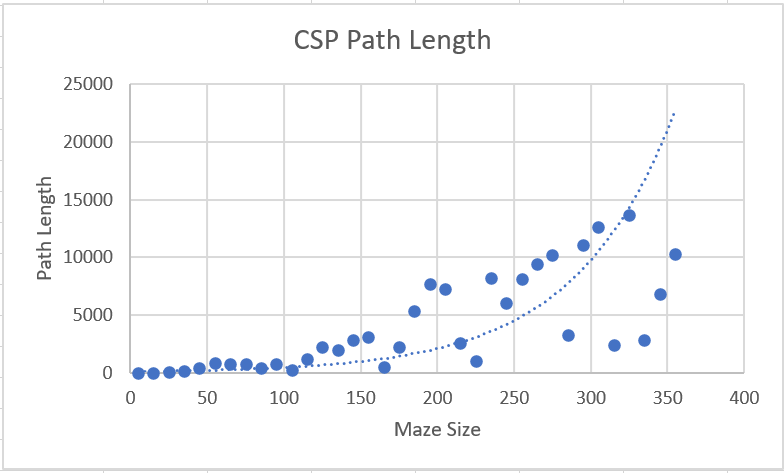
\includegraphics[scale=0.5]{assets/CSPPathVsSize.PNG}
                \caption{Model checking steps vs maze size}
            \end{subfigure}
            \begin{subfigure}{.5\textwidth}
                \centering
                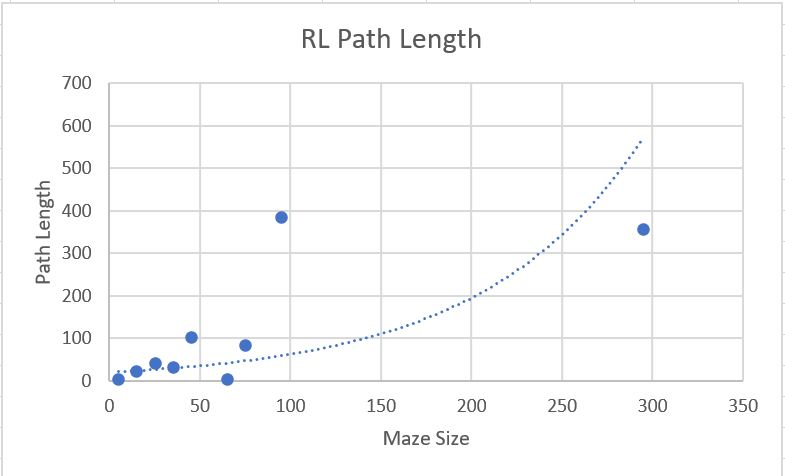
\includegraphics[scale=0.5]{assets/RLPathVsSize.PNG}
                \caption{RL steps vs maze size}
            \end{subfigure}
        \end{figure}

         \tab When the number of steps in the found path is shown on its own, 
         however, it paints a much worse picture for the Q-learning algorithm. 
         It was able to find a path from the start point to the goal in 
         only a few of the maze sizes, whereas CSP (while eventually 
         running out of memory) was able to find a path in every maze 
         it was able to search.

         \tab It is suspected here that Q-learning often failed to find the goal 
         in larger maze sizes due to its reward algorithm. As it proceeded 
         through the maze and its step count for each iteration increased, 
         it became less and less likely to perform the required 'random' 
         movements that were not greedy to escape local optima. This lead
         to it getting stuck in long dead-end paths, where there is a much 
         higher incentive for the algorithm to remain
         in the current state than move back out.

         \tab Different configurations of starting values were tested to try 
         overcoming this problem, such as increasing alpha, gamma, epsilon, 
         the maximum number of steps and the maximum number of iterations. 
         However, none of these were capable of avoiding the issue faced. 
         More max steps meant just more steps where the agent did not move, more
         iterations were ineffective as it behaved the same way each iteration, 
         gamma was already at 0.99 so further increases were un-noticeable, 
         and alpha and epsilon increases did nothing, likely because by the 
         time the algorithm had reached a dead end the chance of backtracking 
         was so low that it was effectively impossible to fix.


         A noteworthy factor for interpreting these results is that RL is
         basically finding a result in the case that it can complete $O(1)$, as
         the results given here were generated under a constant environment for 
         all the solutions. It just looks like $O(n)$ until it hits that wall. 
         This means that the one solution it managed to find
         at around maze size 300x300 is an outlier, and we can see that it
         just managed to be found because the solution was so close. On the
         other hand, DFS still managed to take a really roundabout path to find
         it.

        \begin{figure}[ht]
            \begin{subfigure}{.5\textwidth}
                \centering
                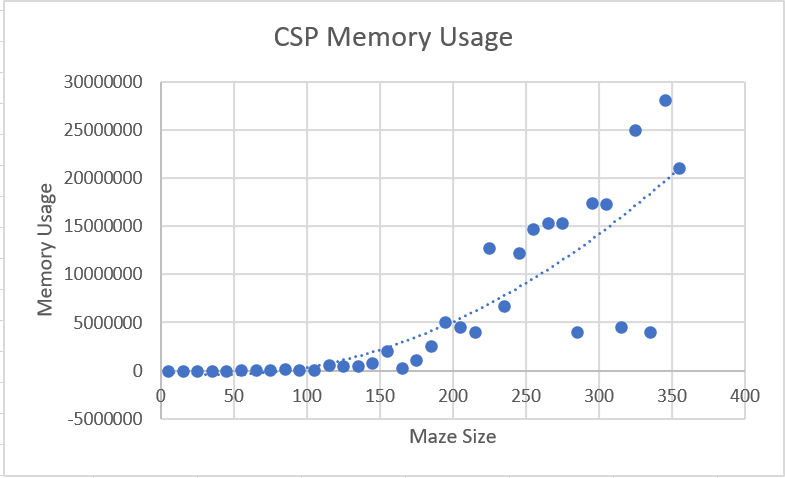
\includegraphics[scale=0.5]{assets/CSPMemoryVsSize.PNG}
                \caption{Model checking memory vs size}
            \end{subfigure}
            \begin{subfigure}{.5\textwidth}
                \centering
                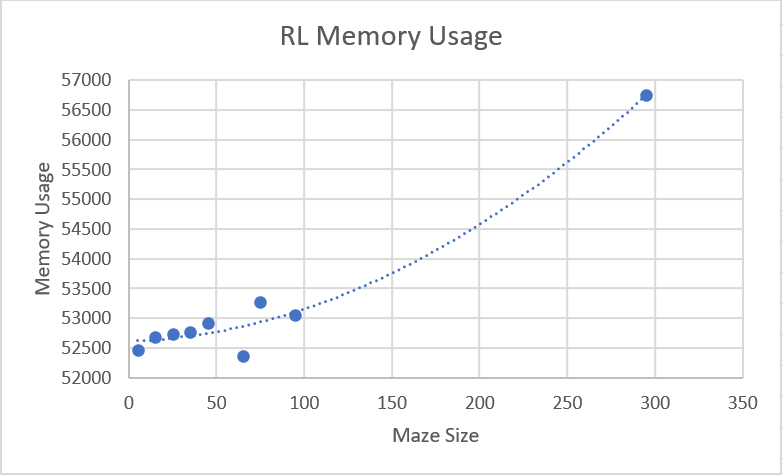
\includegraphics[scale=0.5]{assets/RlMemoryVsSize.PNG}
                \caption{RL memory vs size}
                \label{sonarCode}
            \end{subfigure}
        \end{figure}

         \tab This graph shows the difference in memory usage between RL and CSP. 
         This is to be expected, as DFS is an exhaustive search, which holds 
         all of the current nodes for the path currently being checked in 
         memory. While more memory efficient than BFS, it is still very 
         memory hungry, but well-worth the results considering the 
         performance of RL.

    \section{Conclusion}\label{sec:conclusion}

        \tab In testing for this report, it is clear that Q-learning does not 
        perform as well as CSP for this task at such high maze sizes. 
        It was consistently faster, less memory intensive and more accurate 
        than CSP at smaller maze sizes, however the algorithm could not perform 
        at higher maze sizes, failing to find paths at all.

        \tab It is advised that the reinforcement learning algorithm be adjusted
        to be dynamic (scaling the variables based on the maze size), and
        introducing a random restart algorithm to it. An alternative to random
        restart would be to just introduce a penalty for repeatedly entering the
        same states, or rewarding it for finding new ones. With these, it is
        potentially possible to keep an $O(n)$ time complexity solving the maze at
        larger mazes as well.
        \\ \\
        If a solution were to be required for deployment using identical 
        configurations to those used in this report, it is recommended that 
        Q-learning be used for smaller maze sizes (for example, below 50) and 
        CSP be used for maze sizes that are larger.

%==============================================================================
    \bibliographystyle{apalike}
    \bibliography{biblio}
\end{document}
